\section{Nutritional Labels for Algorithmic Rankers}
\label{sec:rankingFacts}
% RankingFacts, with the different facets of explanation

To make our discussion more concrete, we now describe \rf, a system that automatically derives nutritional labels for rankings~\cite{DBLP:conf/sigmod/YangSAHJM18}. 
%
Algorithmic decisions often result in scoring and ranking individuals --- to determine credit worthiness, desirability for college admissions and employment, and compatibility as dating partners.   Algorithmic rankers take a collection of items as input and produce a ranking – a sorted list of items – as output. The simplest kind of a ranker is a score-based ranker, which computes a score for each item independently, and then sorts the items on their scores.  While automatic and seemingly objective, rankers can discriminate against individuals and protected groups~\cite{CitronP14}, and exhibit low diversity at top ranks~\cite{DBLP:conf/edbt/StoyanovichAM11}. Furthermore, ranked results are often unstable --- small changes in the input or in  the ranking methodology may lead to drastic changes in the output, making the result uninformative and easy to manipulate~\cite{gladwell}.  Similar concerns apply in cases where items other than individuals are ranked, including colleges, academic departments, and products.

\begin{figure*}[t!]	
\centering
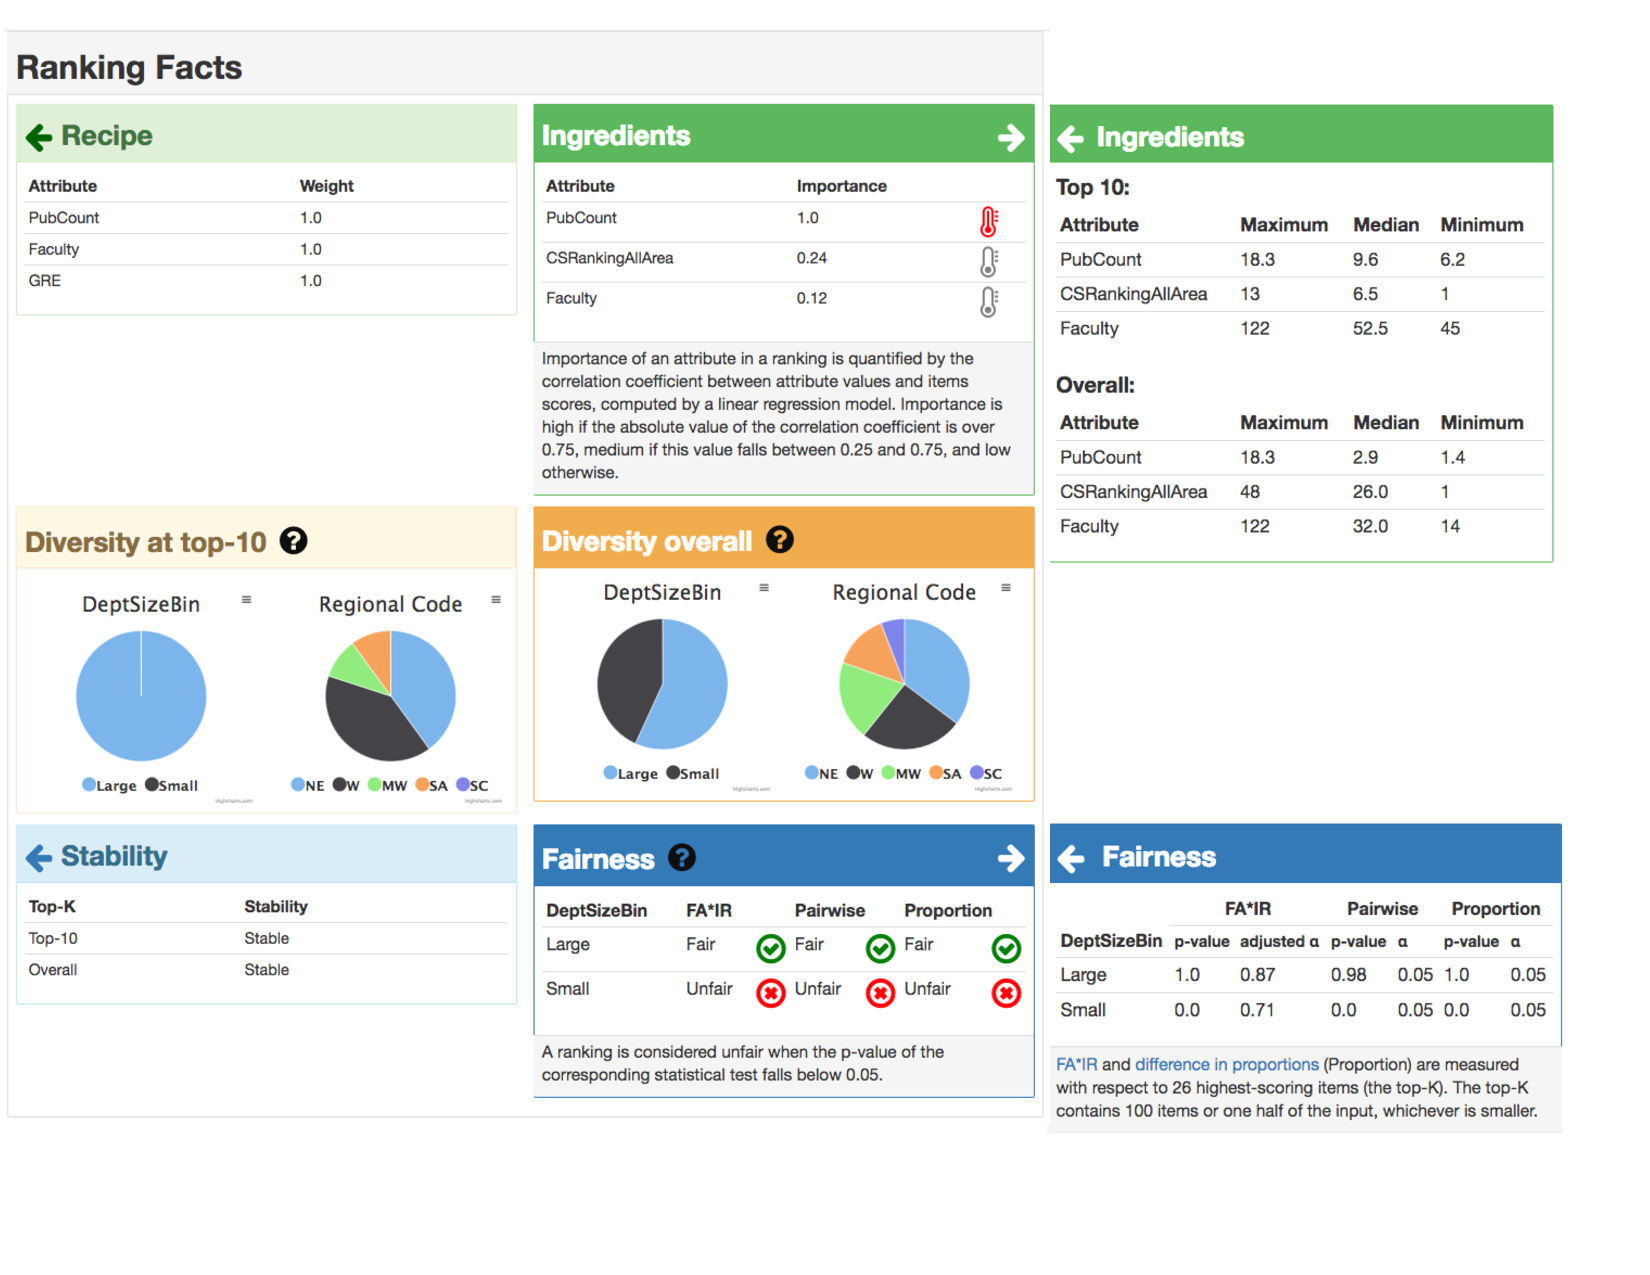
\includegraphics[width=\linewidth]{figs/label.pdf}
     \caption{\rf for the CS departments dataset. The Ingredients widget (green) has been expanded to show the details of the attributes that strongly influence the ranking.  The Fairness widget (blue) has been expanded to show the computation that produced the fair/unfair labels.}
     \label{fig:label}
\end{figure*}

In a recent work, we developed \rf, a nutritional label for rankings~\cite{DBLP:conf/sigmod/YangSAHJM18}.    \rf is available as a Web-based tool\footnote{\url{http://demo.dataresponsibly.com/rankingfacts/}}, and its code is available in the open source~\footnote{\url{https://github.com/DataResponsibly/RankingFacts}}.  Figure~\ref{fig:label} presents \rf~that explains a ranking of Computer Science departments.  The data in this example was obtained from CS Rankings\footnote{\url{https://github.com/emeryberger/CSRankings}}, augmented with attributes from the NRC dataset~\footnote{\url{http://www.nap.edu/rdp/}}.
\rf is made up of a collection of visual widgets, each with an overview and a detailed view.  Each widget addresses an essential aspect of transparency and interpretability, and is based on our recent technical work on fairness~\cite{DBLP:conf/sigmod/AsudehJS019,DBLP:conf/ssdbm/YangS17},  diversity~\cite{diversity,DBLP:conf/edbt/StoyanovichAM11,DBLP:conf/edbt/StoyanovichYJ18,DBLP:conf/ijcai/YangGS19}, and stability~\cite{DBLP:journals/pvldb/AsudehJMS18} in algorithmic rankers.   We now describe each widget in some detail.

\subsection{Recipe and Ingredients}

These two widgets help to explain the ranking methodology.  The {\sf Recipe} widget succinctly describes the ranking algorithm.  For example, for a linear scoring formula, each attribute would be listed together with its weight. The {\sf Ingredients} widget lists attributes most material to the ranked outcome, in order of importance.  For example, for a linear model, this list could present the attributes with the highest learned weights.  Put another way, the explicit intentions of the designer of the scoring function about which attributes matter, and to what extent, are stated in the {\sf Recipe}, while {\sf Ingredients} may show  attributes that are actually associated with high rank.  Such associations can be derived with linear models or with other methods, such as rank-aware similarity in our prior work~\cite{DBLP:conf/edbt/StoyanovichAM11}. The detailed {\sf Recipe} and {\sf Ingredients} widgets list statistics of the attributes in the {\sf Recipe} and in the {\sf Ingredients}: minimum, maximum and median values at the top-$10$ and over-all.

\subsection{Stability}
\label{sec:sys:stab}

The {\sf Stability} widget explains whether the ranking methodology is robust on this particular dataset.  An unstable ranking is one where slight changes to the data (\eg due to uncertainty and noise), or to the methodology (\eg by slightly adjusting the weights in a score-based ranker) could lead to a significant change in the output. This widget reports a stability score, as a single number that indicates the extent of the change required for the ranking to change.  As with the widgets above, there is a detailed {\sf Stability} widget to complement the overview widget.  

An example is shown in Figure~\ref{fig:stability}, where the stability of the ranking is quantified as the slope of the line that is fit to the score distribution, at the top-$10$ and over-all.  A score distribution is unstable if scores of items in adjacent ranks are close to each other, and so a very small change in scores will lead to a change in the ranking.  In this example the score distribution is considered unstable if the slope is 0.25 or lower.  Alternatively, stability can be computed with respect to each scoring attribute, or it can be assessed using a model of uncertainty in the data.  In these cases, stability quantifies the extent to which a ranked list will change as a result of small changes to the underlying data.  A complementary notion of stability quantifies the magnitude of change as a result of small changes to the ranking model.  We explored this notion in our recent work, briefly discussed below.

In~\cite{DBLP:journals/pvldb/AsudehJMS18} we develped methods for quantifying the stability of a score-based ranker with respect to a given dataset.  Specifically, we considered rankers that specify non-negative weights, one for each item attribute, and compute the score as a weighted sum of attribute values. We focused on a notion of stability that quantifies whether the output ranking will change due to a small change in the attribute weights.  This notion of stability is  natural  for consumers of a ranked list (\ie those who use the ranking to prioritize items and make decisions), who should be able to assess the magnitude of the {\em region in the weight space} that produces the observed ranking.  If this region is large, then the same ranked order would be obtained for many choices of weights, and the ranking is stable.  But if this region is small, then we know that only a few weight choices can produce the observed ranking.  This may suggest that the ranking was engineered or ``cherry-picked'' by the producer to obtain a specific outcome.

%If a ranking is stable,  then the same ranking would be obtained for many choices of weights. But if this region is small, then we know that only a few weight choices can produce the observed ranking. This may suggest that the ranking was engineered or “cherry-picked” by the producer to obtain a specific outcome.  Human experts who produce scoring functions for generating the rankings desire to produce stable results.  We argued in [31] that stability in a ranked output is an important aspect of algorithmic transparency, because it allows the producer to justify their ranking methodology, and to gain the trust of consumers.


\subsection{Fairness}
\label{sec:sys:fair}

\begin{figure}[t!]	
\centering
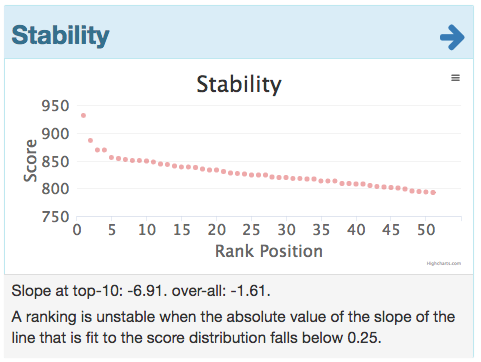
\includegraphics[width=3in]{figs/stability.png}
     \caption{{\sf Stability}: detailed widget.}
     \label{fig:stability}
\end{figure}

The {\sf Fairness} widget quantifies whether the ranked output exhibits statistical parity (one interpretation of fairness) with respect to one or more sensitive attributes, such as gender or race of individuals~\cite{DBLP:conf/ssdbm/YangS17}.  We denote one or several values of the sensitive attribute as a protected feature.  For example, for the sensitive attribute {\sf gender}, the assignment {\sf gender=F} is a protected feature.

A variety of fairness measures have been proposed in the literature~\cite{DBLP:journals/datamine/Zliobaite17}, with a primary focus on classification or risk assessment tasks. One typical fairness measure for classification compares the proportion of members of a protected group (\eg female gender or minority race) who receive a positive outcome to their proportion in the overall population.  For example, if the dataset contains an equal number of men and women, then among the individuals invited for a job interview, one half should be women.  A measure of this kind can be adapted to rankings by quantifying the proportion of members of a protected group in some selected set of size $k$ (treating the top-$k$ as a set).

In~\cite{DBLP:conf/ssdbm/YangS17}, we were the first to propose a family of {\em fairness measures specifically for rankings}.  Our measures are based on a generative process for rankings that meet a particular fairness criterion (fairness probability $f$) and are drawn from a dataset with a given proportion of members of a binary protected group ($p$). This method was subsequently used in FA*IR~\cite{DBLP:conf/cikm/ZehlikeB0HMB17} to quantify fairness in every prefix of a top-$k$ list.  We also developed a pairwise measure that directly models the probability that a member of a protected group is preferred to a member of the non-protected group.

Let us now return to the {\sf Fairness} widget in Figure~\ref{fig:label}.  We select a binary version of the department size attribute {\sf DeptSizeBin} from the CS departments dataset as the sensitive attribute, and treat the value and ``small'' as the protected feature.  The summary view of the {\sf Fairness} widget in our example presents the output of three fairness measures: FA*IR~\cite{DBLP:conf/cikm/ZehlikeB0HMB17}, proportion~\cite{DBLP:journals/datamine/Zliobaite17}, and our own pairwise measure.  All these measures are statistical tests, and whether a result is fair is determined by the computed $p$-value.  The detailed {\sf Fairness} widget provides additional information about the tests and explains the process.

\subsection{Diversity}
\label{sec:sys:div}

Fairness is related to diversity: ensuring that different kinds of objects are represented in the output of an algorithmic process~\cite{diversity}.  Diversity has been considered in search and recommender systems, but in a narrow context, and was rarely applied to profiles of individuals. % We are currently working on defining diversity measures for ranked outputs, based on our work in~\cite{diversity,DBLP:conf/edbt/StoyanovichAM11}. 
%
The {\sf Diversity} widget  shows diversity with respect to a set of demographic categories of individuals, or a set of categorical attributes of other kinds of items~\cite{diversity}.  The widget displays the proportion of each category in the top-$10$ ranked list and over-all, and, like other widgets, is updated as the user selects different ranking methods or sets different weights.  In our example in Figure~\ref{fig:label}, we quantify diversity with respect to department size and to the regional code of the university.  By comparing the pie charts for top-$10$ and over-all, we observe that only large departments are present in the top-$10$.

This simple diversity measure that is currently included in \rf can be augmented by, or replaced with, other measures, including, for example, those we developed in our recent work~\cite{DBLP:conf/edbt/StoyanovichYJ18,DBLP:conf/ijcai/YangGS19}.
